% AST2000 Part 7: the landing (partial paper: abstract, results, discussion and conclusions, figures, flowchart).
% The star exercise (challenge D) is the separate document part7_star.tex.
% Compile: cd "Project 7/paper" && latexmk -pdf part7.tex   (or: python build_papers.py 7 from the repo root)
% Every number written as \val{key} comes from results.tex, made by pro_7.py.
\documentclass[aps,prd,twocolumn,nofootinbib,floatfix,superscriptaddress]{revtex4-2}
\usepackage{../../common/paper/ast2000}
\usepackage{tikz}
\usetikzlibrary{arrows.meta,positioning,shapes.geometric}
\tikzset{
  box/.style={draw, rounded corners=2pt, align=center, font=\footnotesize, inner sep=3pt, text width=#1},
  box/.default=6.6cm,
  decision/.style={draw, diamond, aspect=2.6, align=center, font=\footnotesize, inner sep=1pt},
  flow/.style={-{Stealth[length=2mm]}, thick}}

\begin{document}

\title{Part 7: Landing on Planet 1}
\author{Sakarias Frette}
\affiliation{AST2000 Rerun, University of Oslo}
\date{\today}

\begin{abstract}
We landed a \val{lander-mass}\,kg lander on planet 1, \val{miss-km}\,km \val{miss-dir} of the site chosen in Part 6, at \val{v-touch}\,m/s (limit \val{v-safe}\,m/s), in full daylight with the star \val{sun-land}$^\circ$ above the horizon.
\begin{itemize}
\item \textbf{Analysis.} In air that co-rotates with the planet, a parachute of at least \val{A-safe}\,m$^2$ brings the lander below \val{v-safe}\,m/s. Without one it would hit the ground at \val{vt-lander}\,m/s.
\item \textbf{Simulator.} Our own descent simulator includes gravity, drag in the rotating air, the lander release and the parachute. It agrees with \code{ast2000tools}~\cite{ast2000tools} to \val{valid-diff}\,m over a whole test descent.
\item \textbf{The landing.} The lander is released from the low orbit with \val{deorbit-dv}\,m/s against its motion and brakes from \val{v-rel-orbit}\,km/s in the upper atmosphere. A \val{chute-area}\,m$^2$ parachute opens \val{chute-height}\,km above the ground. The release time comes from a root search with our simulator, and the real flight landed within \val{plan-miss-km}\,km of the predicted point.
\item \textbf{Margins.} The peak drag per area was \val{burn-margin} times below the burn-up limit. The parachute's peak load was \val{chute-peak}\,kN, against a 250\,kN limit.
\end{itemize}
\end{abstract}

\maketitle

% =====================================================================
\section{Results}
\subsection{Air resistance and terminal velocity}
We use the drag model of the assignment~\cite{ast2000project}.
The atmosphere co-rotates with the planet, so the air at $\vb r$ moves with $\vb w=\omega\hat{\vb z}\times\vb r$, which is \val{w-equator}\,m/s at the equator.
Drag acts on the velocity relative to the air, $\vb v_{\rm drag}=\vb v-\vb w$:
\begin{equation}
  \vb F_d=-\tfrac12\rho(h)C_dA\,|\vb v_{\rm drag}|\,\vb v_{\rm drag},\qquad C_d=1 .
\end{equation}
Two facts follow from this.
\begin{itemize}
\item The drag always opposes the relative velocity, and gravity is radial. Nothing sustains a tangential relative velocity, so $v_\theta\to0$ relative to the air.
\item Drag grows as $v^2$ until it balances gravity, so $v_r$ settles at the terminal velocity
\begin{equation}
  v_t=\sqrt{\frac{2GMm}{\rho AR^2}}\quad\Longrightarrow\quad A=\frac{2GMm}{\rho_0R^2v^2}.
\end{equation}
\end{itemize}
For our lander:
\begin{itemize}
\item Alone it lands at $v_t=\val{vt-lander}$\,m/s, which would be a crash.
\item A total area of \val{A-safe}\,m$^2$ gives exactly \val{v-safe}\,m/s (\cref{fig:terminal}).
\item Opening at terminal speed, the parachute's drag is $mg\,A_{\rm tot}/A_{\rm lander}$. The largest chute that survives opening is therefore \val{A-max}\,m$^2$.
\item Thrusters alone would need $F_L=\tfrac12\rho_0A(v_t^2-v_{\rm safe}^2)=\val{FL-lander}$\,N, almost the lander's weight (\cref{fig:thrusters}).
\end{itemize}
We use a \val{chute-area}\,m$^2$ parachute, sized for \val{v-target}\,m/s at the ground, \val{thruster-text}.

\widefig{a1_terminal_velocity}{Terminal velocity against height for the lander with parachutes of several sizes, and the area needed for a given landing speed.}{fig:terminal}
\colfig{a2_thrusters}{Thruster force needed for a \val{v-safe}\,m/s touchdown against the total area.}{fig:thrusters}

\subsection{The simulator}
Our simulator (\cref{fig:flow}) integrates gravity, drag in the co-rotating air (density from the Part 6 model), the lander release, the parachute and the thrusters.
It uses an adaptive eighth-order Runge--Kutta solver (DOP853~\cite{dormand1980}), and the ground is detected as an event.
The adaptive steps handle the violent moments automatically: entry, the parachute opening, decelerations of $\sim$100\,$g$.
On a test descent (release with \val{valid-dv}\,m/s, \val{valid-chute}\,m$^2$ parachute at \val{valid-chute-height}\,km) it agrees with \code{ast2000tools} to within 20\,m before entry and \val{valid-diff}\,m after (\cref{fig:validation}).
The remaining difference matches the 1--2\% between our density model and the API's (Part 6).

\begin{figure}[tbp]\centering
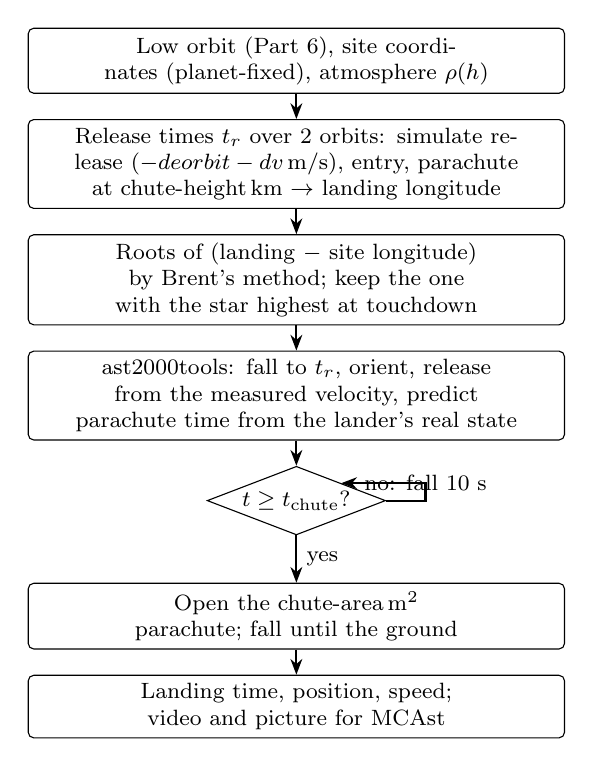
\begin{tikzpicture}[node distance=3.2mm]
\node[box] (start) {Low orbit (Part 6), site coordinates (planet-fixed), atmosphere $\rho(h)$};
\node[box, below=of start] (scan) {Release times $t_r$ over 2 orbits: simulate release ($-\val{deorbit-dv}$\,m/s), entry, parachute at \val{chute-height}\,km $\to$ landing longitude};
\node[box, below=of scan] (root) {Roots of (landing $-$ site longitude) by Brent's method; keep the one with the star highest at touchdown};
\node[box, below=of root] (fly) {\code{ast2000tools}: fall to $t_r$, orient, release from the measured velocity, predict parachute time from the lander's real state};
\node[decision, below=of fly] (chute) {$t\ge t_{\rm chute}$?};
\node[box, below=6mm of chute] (open) {Open the \val{chute-area}\,m$^2$ parachute; fall until the ground};
\node[box, below=of open] (out) {Landing time, position, speed; video and picture for MCAst};
\draw[flow] (start) -- (scan); \draw[flow] (scan) -- (root); \draw[flow] (root) -- (fly); \draw[flow] (fly) -- (chute);
\draw[flow] (chute) -- node[right, font=\footnotesize] {yes} (open);
\draw[flow] (chute.east) -- ++(0.5,0) node[above, font=\footnotesize] {no: fall 10 s} |- (chute.north east);
\draw[flow] (open) -- (out);
\end{tikzpicture}
\caption{Flowchart of the landing code.}\label{fig:flow}
\end{figure}

\widefig{b1_validation}{Our simulator against \code{ast2000tools} on a test descent: height, speed relative to the air, and the distance between the two.}{fig:validation}

\subsection{The landing}
The lander's landing longitude depends on when it is released.
Once braked it drifts with the air, so its planet-fixed position hardly changes afterwards.
Scanning the release time over two orbits gives \val{n-releases} releases that land on site \val{site-index} (\cref{fig:release}).
We take the one in sunlight: release at $t=\val{t-release}$\,h.

In the real flight, the spacecraft oriented itself at that time and released the lander with \val{deorbit-dv}\,m/s against its measured velocity (\cref{fig:descent}).
\begin{itemize}
\item \textbf{Braking:} it slowed from \val{v-rel-orbit}\,km/s high in the atmosphere, at a peak drag per area of \val{max-q}\,Pa, \val{burn-margin} times below the burn-up limit.
\item \textbf{Parachute:} it opened \val{t-chute}\,min after the release, at \val{chute-height}\,km, with a peak load of \val{chute-peak}\,kN.
\item \textbf{Touchdown:} \val{descent-min}\,min after the release, at $t=\val{t-land}$\,h.
\end{itemize}
\code{ast2000tools} reported a successful landing at \val{v-touch}\,m/s, against our prediction of \val{v-touch-plan}\,m/s (\cref{fig:final}).
The landing point is \val{miss-km}\,km \val{miss-dir} of site \val{site-index} along the equator (\cref{fig:ground}), with the star \val{sun-land}$^\circ$ high.
The landing video (\code{landing.xml}) and a picture from the surface (\code{landed.xml}) are in MCAst.

\widefig{c1_release_time}{Landing longitude miss against release time; the chosen release is the star.}{fig:release}
\widefig{c2_descent}{The landing: planned against flown height and speed, drag per area against the burn-up limit, and drag force against the parachute limit.}{fig:descent}
\colfig{c3_final_approach}{The last kilometres: falling speed against height, with the terminal velocity curves.}{fig:final}
\widefig{c4_ground_track}{Where it came down. Planet-fixed view from above the north pole, with day and night at touchdown, and height against distance from the site.}{fig:ground}

% =====================================================================
\section{Discussion and conclusions}
Physics alone made the landing robust: no trial and error was needed.
\begin{itemize}
\item The lander's small area per mass makes it brake high, where the air is thin. The drag per area stays far below the burn-up limit even for a direct entry.
\item Opening the parachute only once the lander falls at its own terminal speed caps the opening load at $mg\,A_{\rm tot}/A_{\rm lander}$, independent of height.
\item Opening it low, at \val{chute-height}\,km, keeps the slow final descent short. Higher openings make the touchdown time, and so the lighting, harder to predict.
\end{itemize}

The landing accuracy comes from two things:
\begin{itemize}
\item a simulator that matches the API to a fraction of a percent of the trip;
\item re-planning from the measured state at release.
\end{itemize}
The remaining \val{plan-miss-km}\,km follows from small differences between our atmosphere model and the API's in the upper atmosphere, where the lander brakes.
This is the same order as the difference measured in Part 6.
A course correction during the parachute phase is not possible.
A smaller miss would need a better density model at 80--120\,km, or iterating the release time against the API.

The lander is on planet 1, on the day side, \val{miss-km}\,km from the chosen site, after touching down at \val{v-touch}\,m/s.

\bibliography{../../common/paper/references}

\end{document}
